\newpage
%***********************************************************************************
\section{Forward Uncertainty Propagation of MCMC samples}\label{app:mcmc_evaluation}
%***********************************************************************************

%-----------------------------------------------------------------------------------------------------
\subsection{FEBA Test No. 214, Cladding Temperature (TC) Output}\label{app:tbl_results_uq_post_tc_214}
%-----------------------------------------------------------------------------------------------------

% FEBA Test No. 214 Posterior Uncertainty Propagation, TC, with model bias term
\rotatebox{90}{\begin{minipage}{0.85\textheight}
    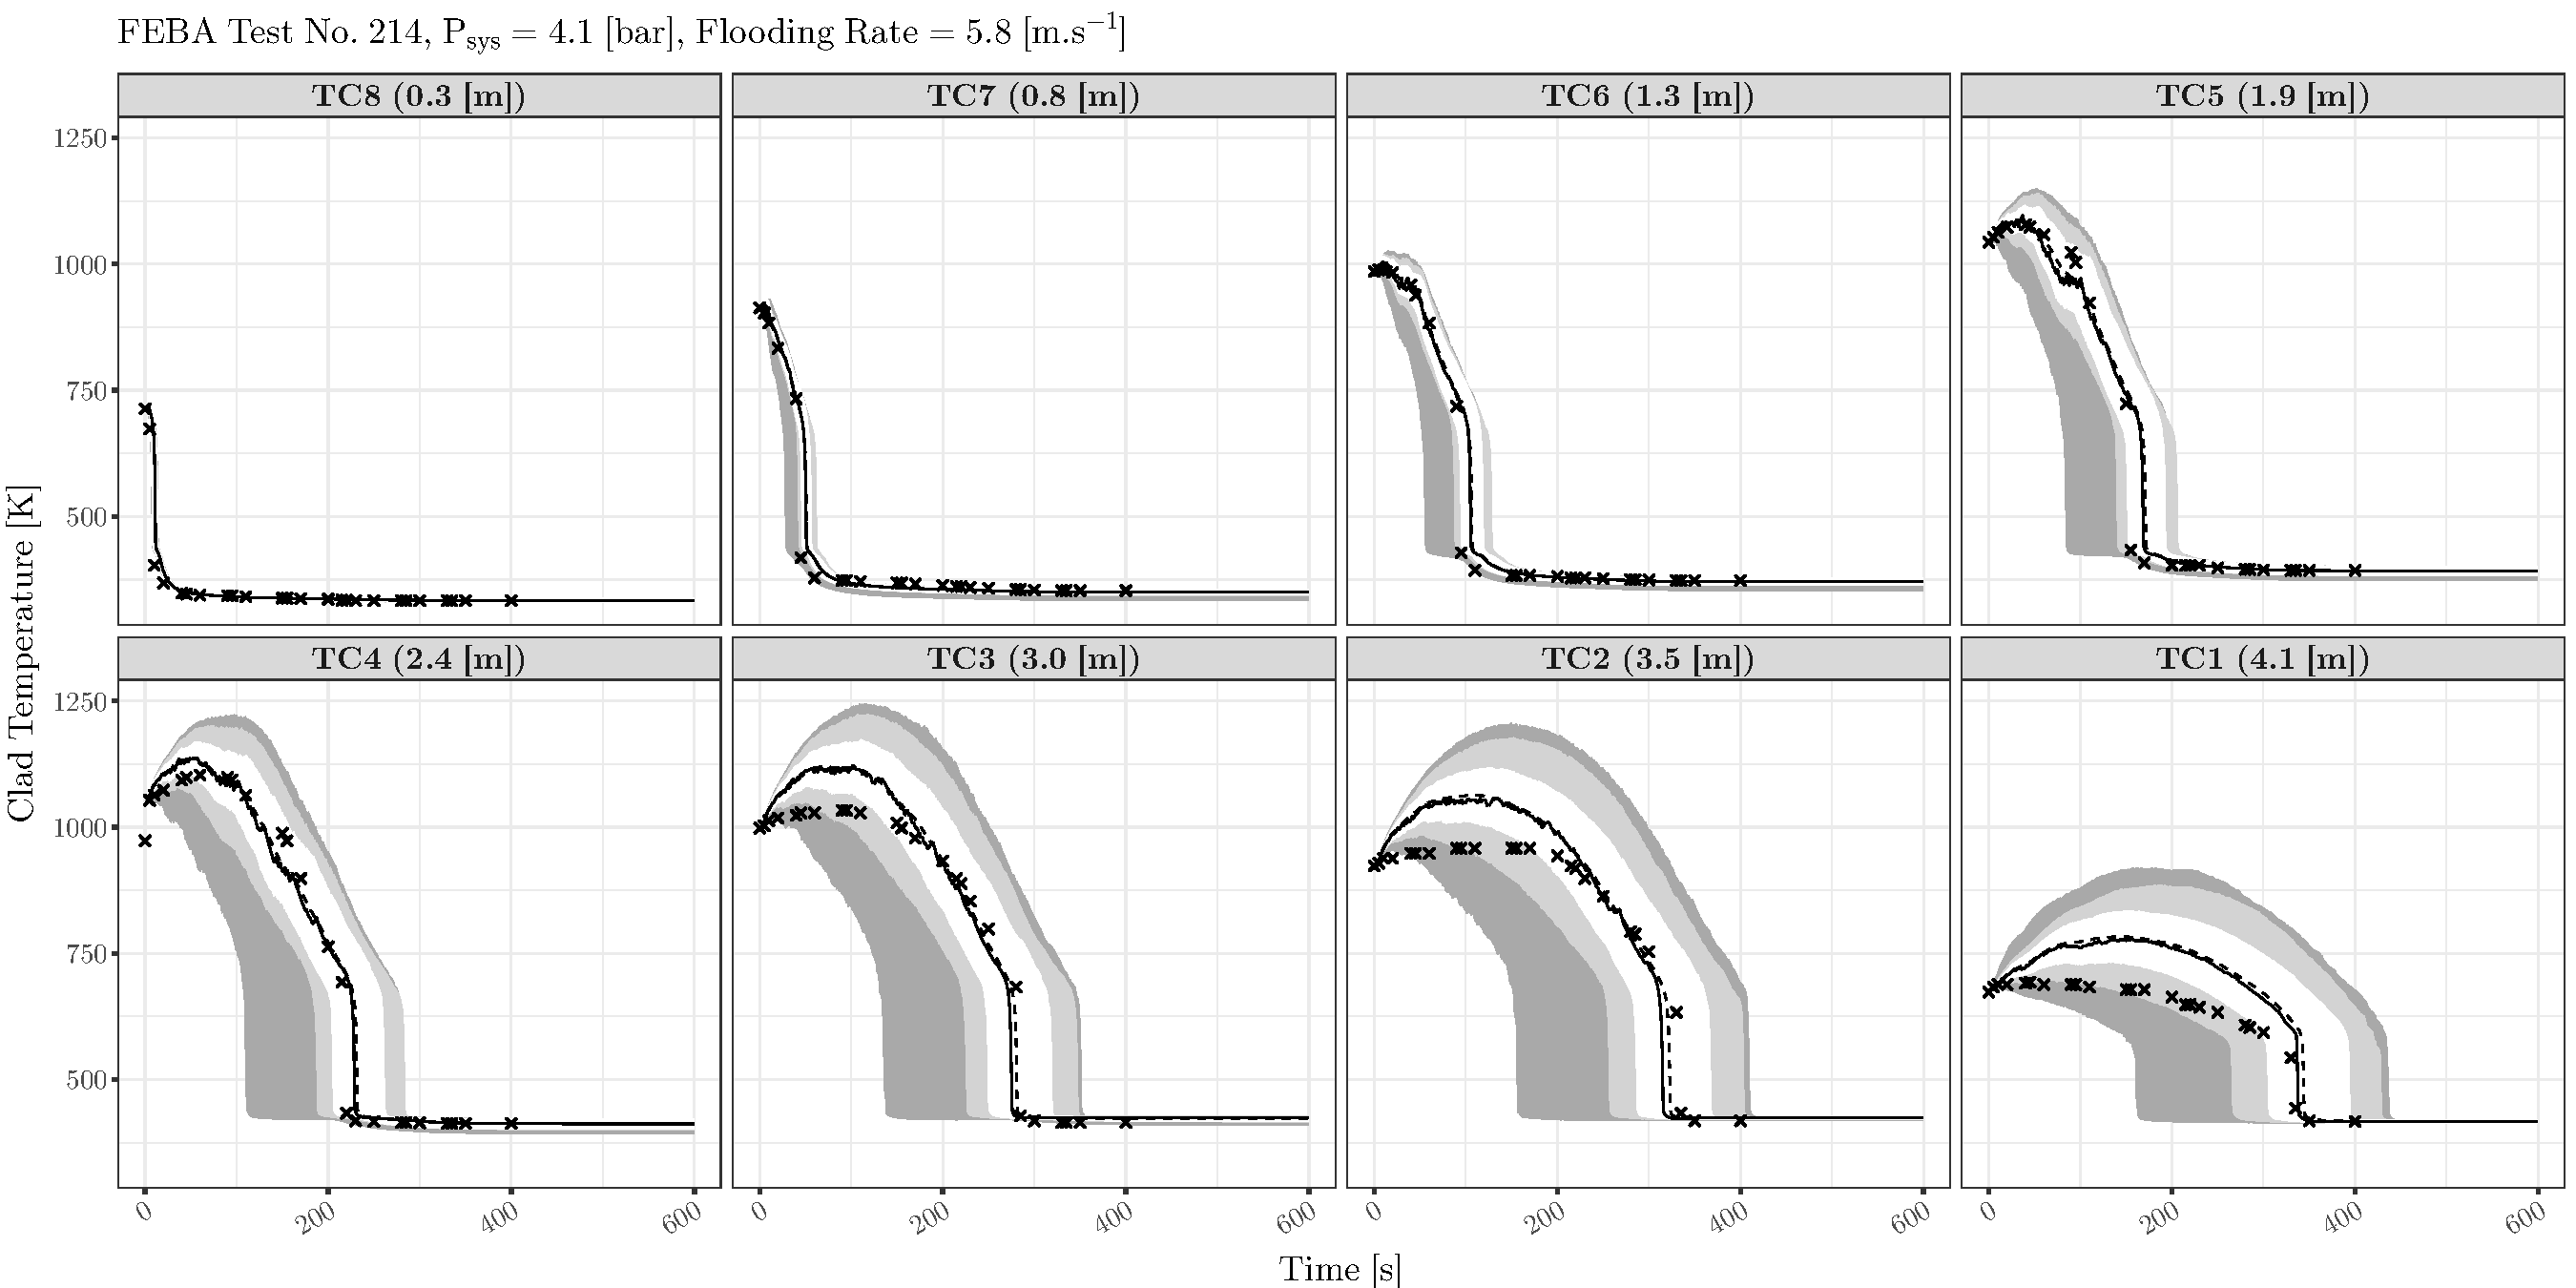
\includegraphics[width=1\textwidth]{../figures/chapter5/figures/plotTraceUQPosteriorAllDiscCenteredTC214}
		\captionof{figure}[Posterior uncertainty propagation of FEBA Test No. $214$ for the cladding temperature output ($TC$). Calibration with model bias term.]{Uncertainty propagation of the parameters uncertainty of \gls[hyper=false]{feba} Test No. $214$ for the cladding temperature output ($TC$) at different axial locations. The uncertainty bounds refer to the symmetric ($95\%$) probability: dark gray, gray, and light gray correspond to the prior, correlated posterior, and independent posterior samples of the parameters, respectively. Solid lines, dashed lines, and crosses indicate the simulation with the nominal parameters values, the median of the posterior uncertainties, and the experimental data, respectively. Posterior samples from calibration with model bias term.}
    \label{fig:ch5_plot_trace_uq_post_tc_214_disc}
\end{minipage}}

% FEBA Test No. 214 Posterior Uncertainty Propagation, TC, without model bias term
\clearpage
\begin{sidewaysfigure}
	\centering
	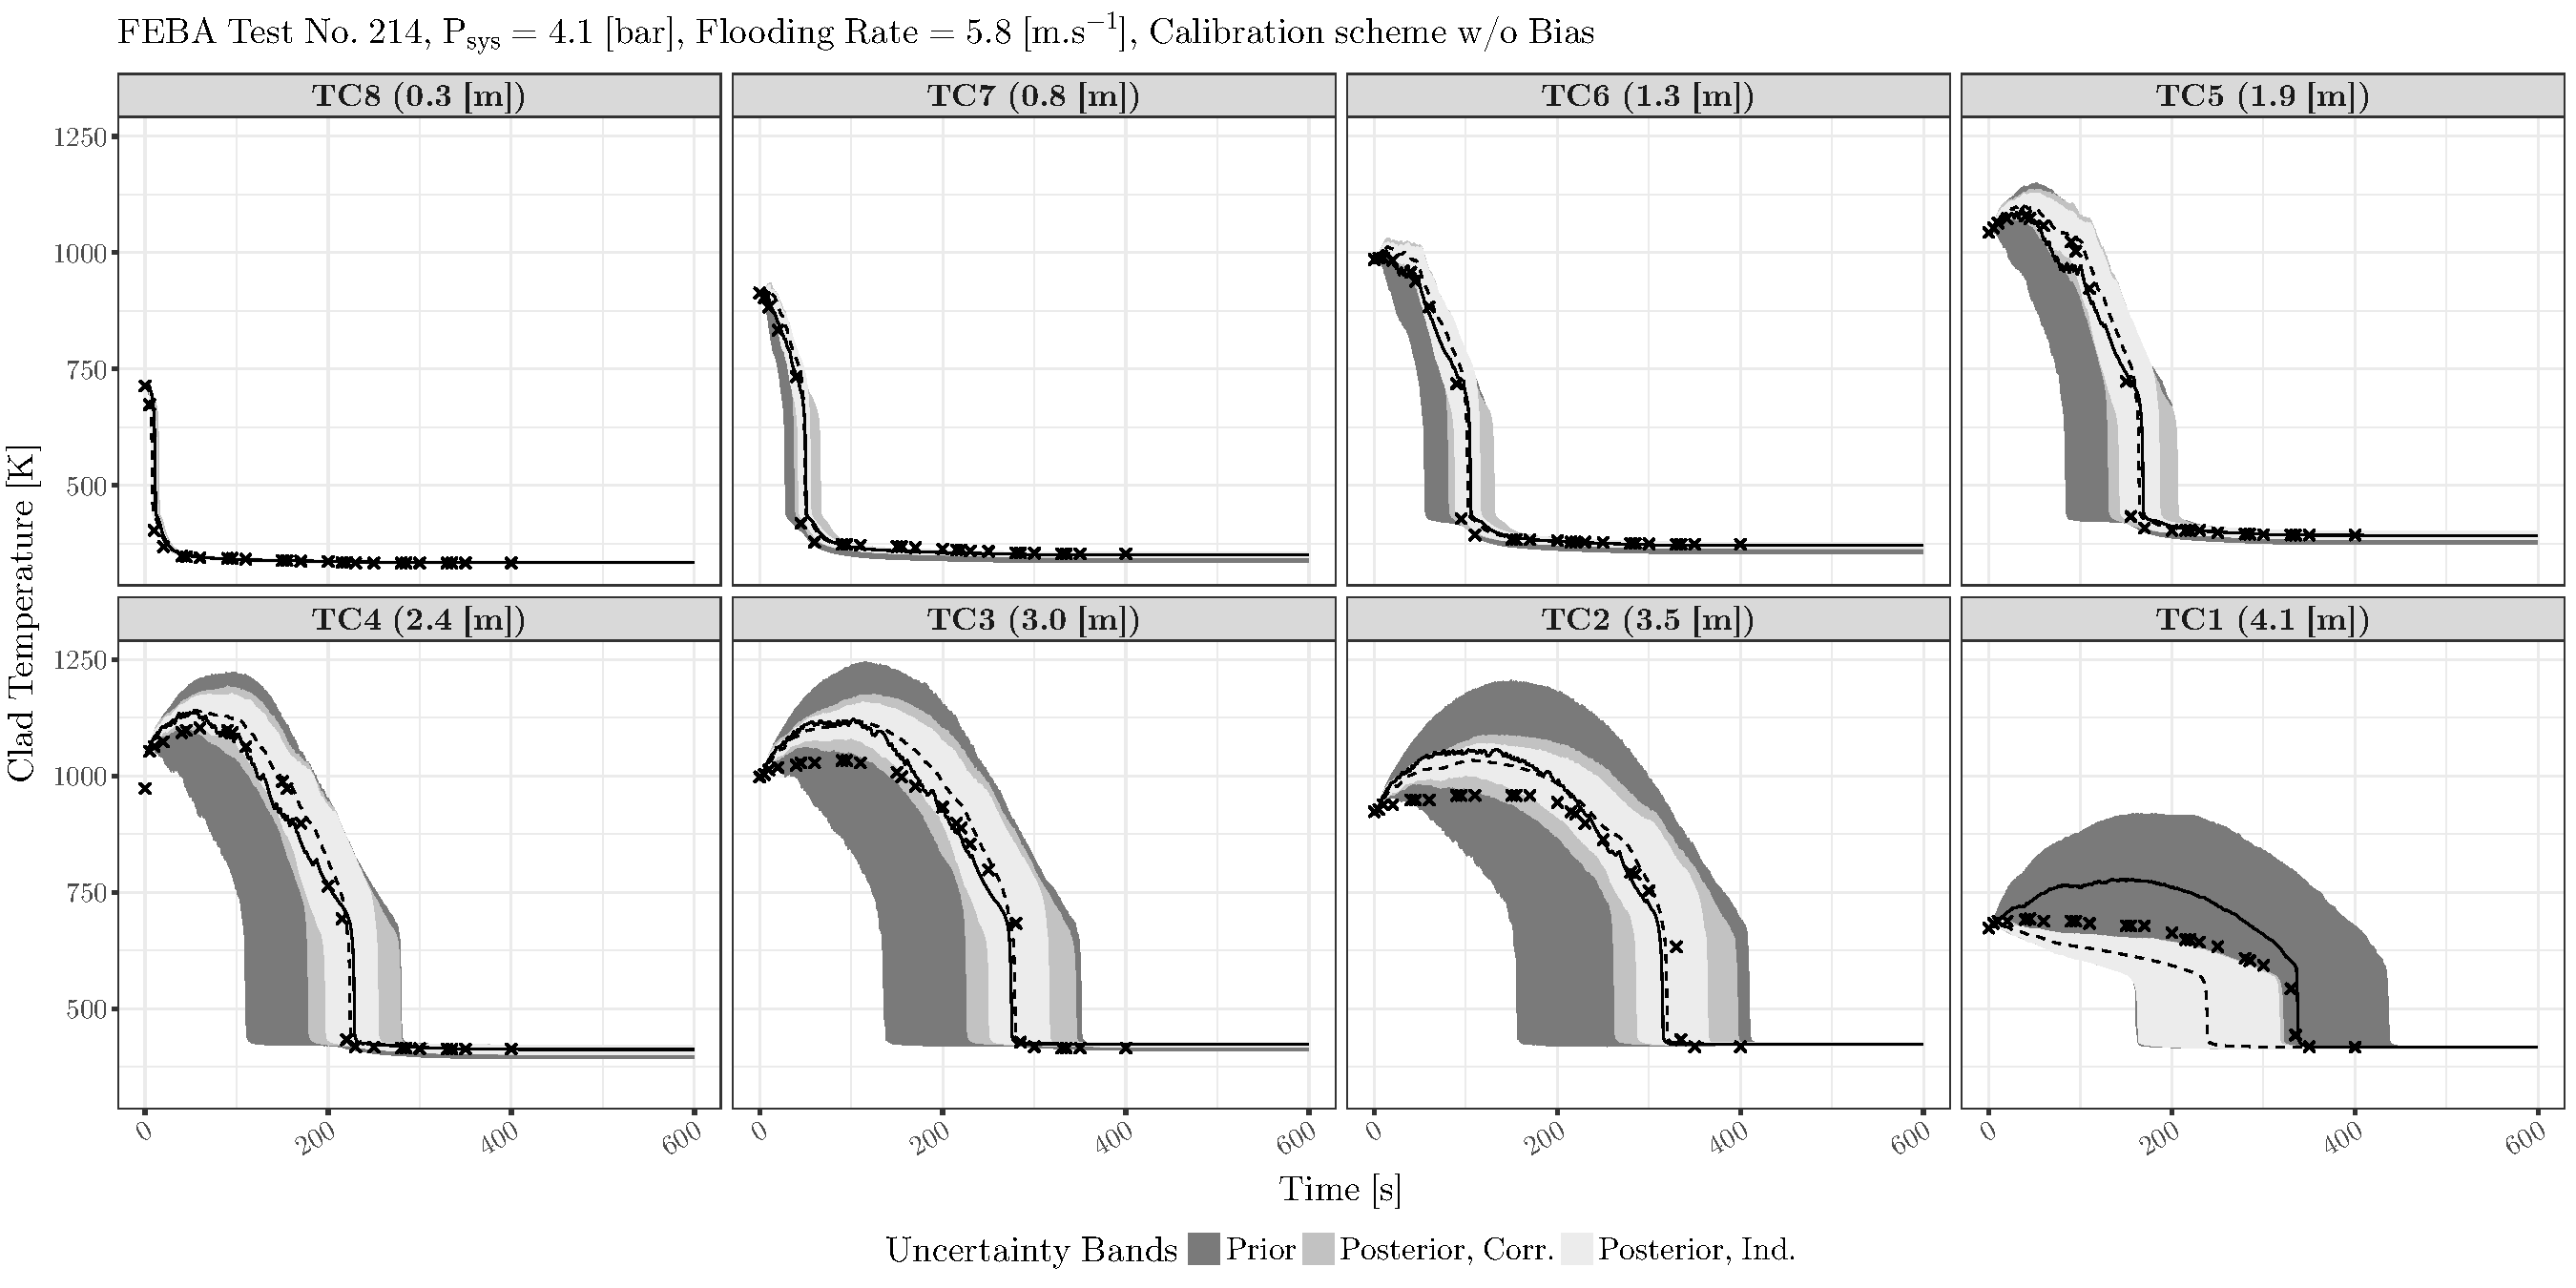
\includegraphics[width=0.90\textwidth]{../figures/chapter5/figures/plotTraceUQPosteriorAllNoDiscNoBCTC214}
		\captionof{figure}[Posterior uncertainty propagation of FEBA Test No. $214$ for the cladding temperature output ($TC$). Calibration without model bias term.]{Uncertainty propagation of the parameters uncertainty of \gls[hyper=false]{feba} Test No. $214$ for the cladding temperature output ($TC$) at different axial locations. The uncertainty bounds refer to the symmetric ($95\%$) probability: dark gray, gray, and light gray correspond to the prior, correlated posterior, and independent posterior samples of the parameters, respectively. Solid lines, dashed lines, and crosses indicate the simulation with the nominal parameters values, the median of the posterior uncertainties, and the experimental data, respectively. Posterior samples from calibration without model bias term.}
	\label{fig:ch5_plot_trace_uq_post_tc_214_nodisc}
\end{sidewaysfigure}
\clearpage

%-----------------------------------------------------------------------------------------------------
\subsection{FEBA Test No. 218, Cladding Temperature (TC) Output}\label{app:tbl_results_uq_post_tc_218}
%-----------------------------------------------------------------------------------------------------

% FEBA Test No. 218 Posterior Uncertainty Propagation, TC, with model bias term
\rotatebox{90}{\begin{minipage}{0.85\textheight}
    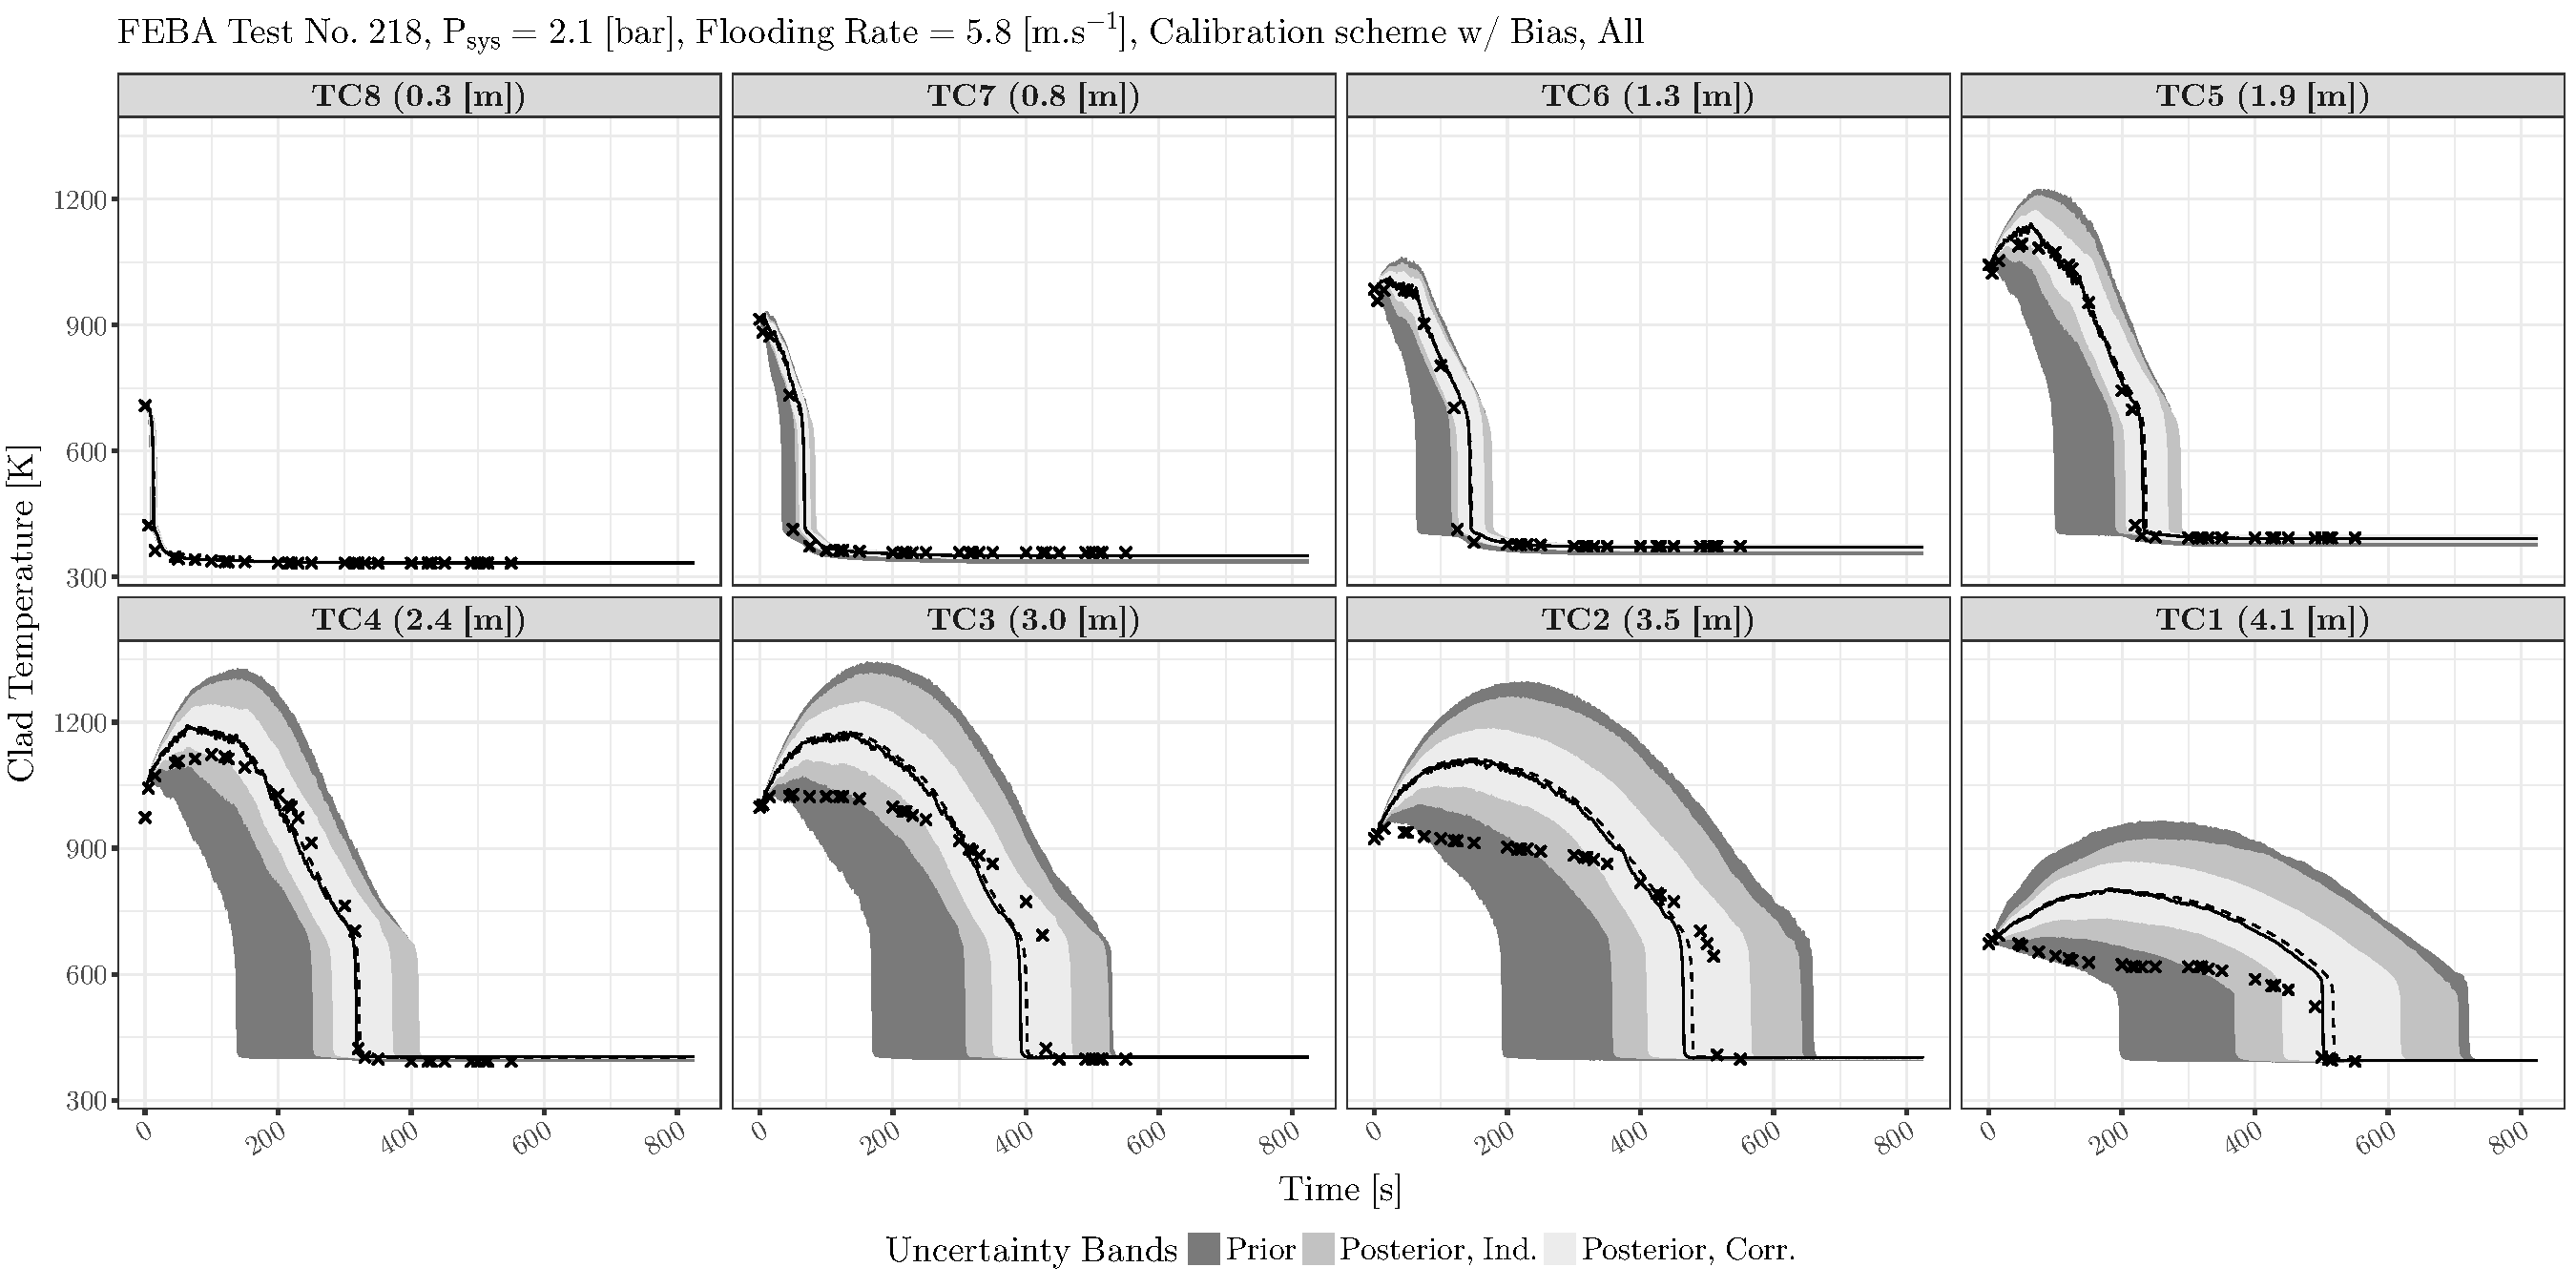
\includegraphics[width=1\textwidth]{../figures/chapter5/figures/plotTraceUQPosteriorAllDiscCenteredTC218}
		\captionof{figure}[Posterior uncertainty propagation of FEBA Test No. $214$ for the cladding temperature output ($TC$). Calibration with model bias term.]{Uncertainty propagation of the parameters uncertainty of \gls[hyper=false]{feba} Test No. $218$ for the cladding temperature output ($TC$) at different axial locations. The uncertainty bounds refer to the symmetric ($95\%$) probability: dark gray, gray, and light gray correspond to the prior, correlated posterior, and independent posterior samples of the parameters, respectively. Solid lines, dashed lines, and crosses indicate the simulation with the nominal parameters values, the median of the posterior uncertainties, and the experimental data, respectively. Posterior samples from calibration with model bias term.}
    \label{fig:ch5_plot_trace_uq_post_tc_218_disc}
\end{minipage}}

% FEBA Test No. 218 Posterior Uncertainty Propagation, TC, without model bias term
\clearpage
\begin{sidewaysfigure}
	\centering
	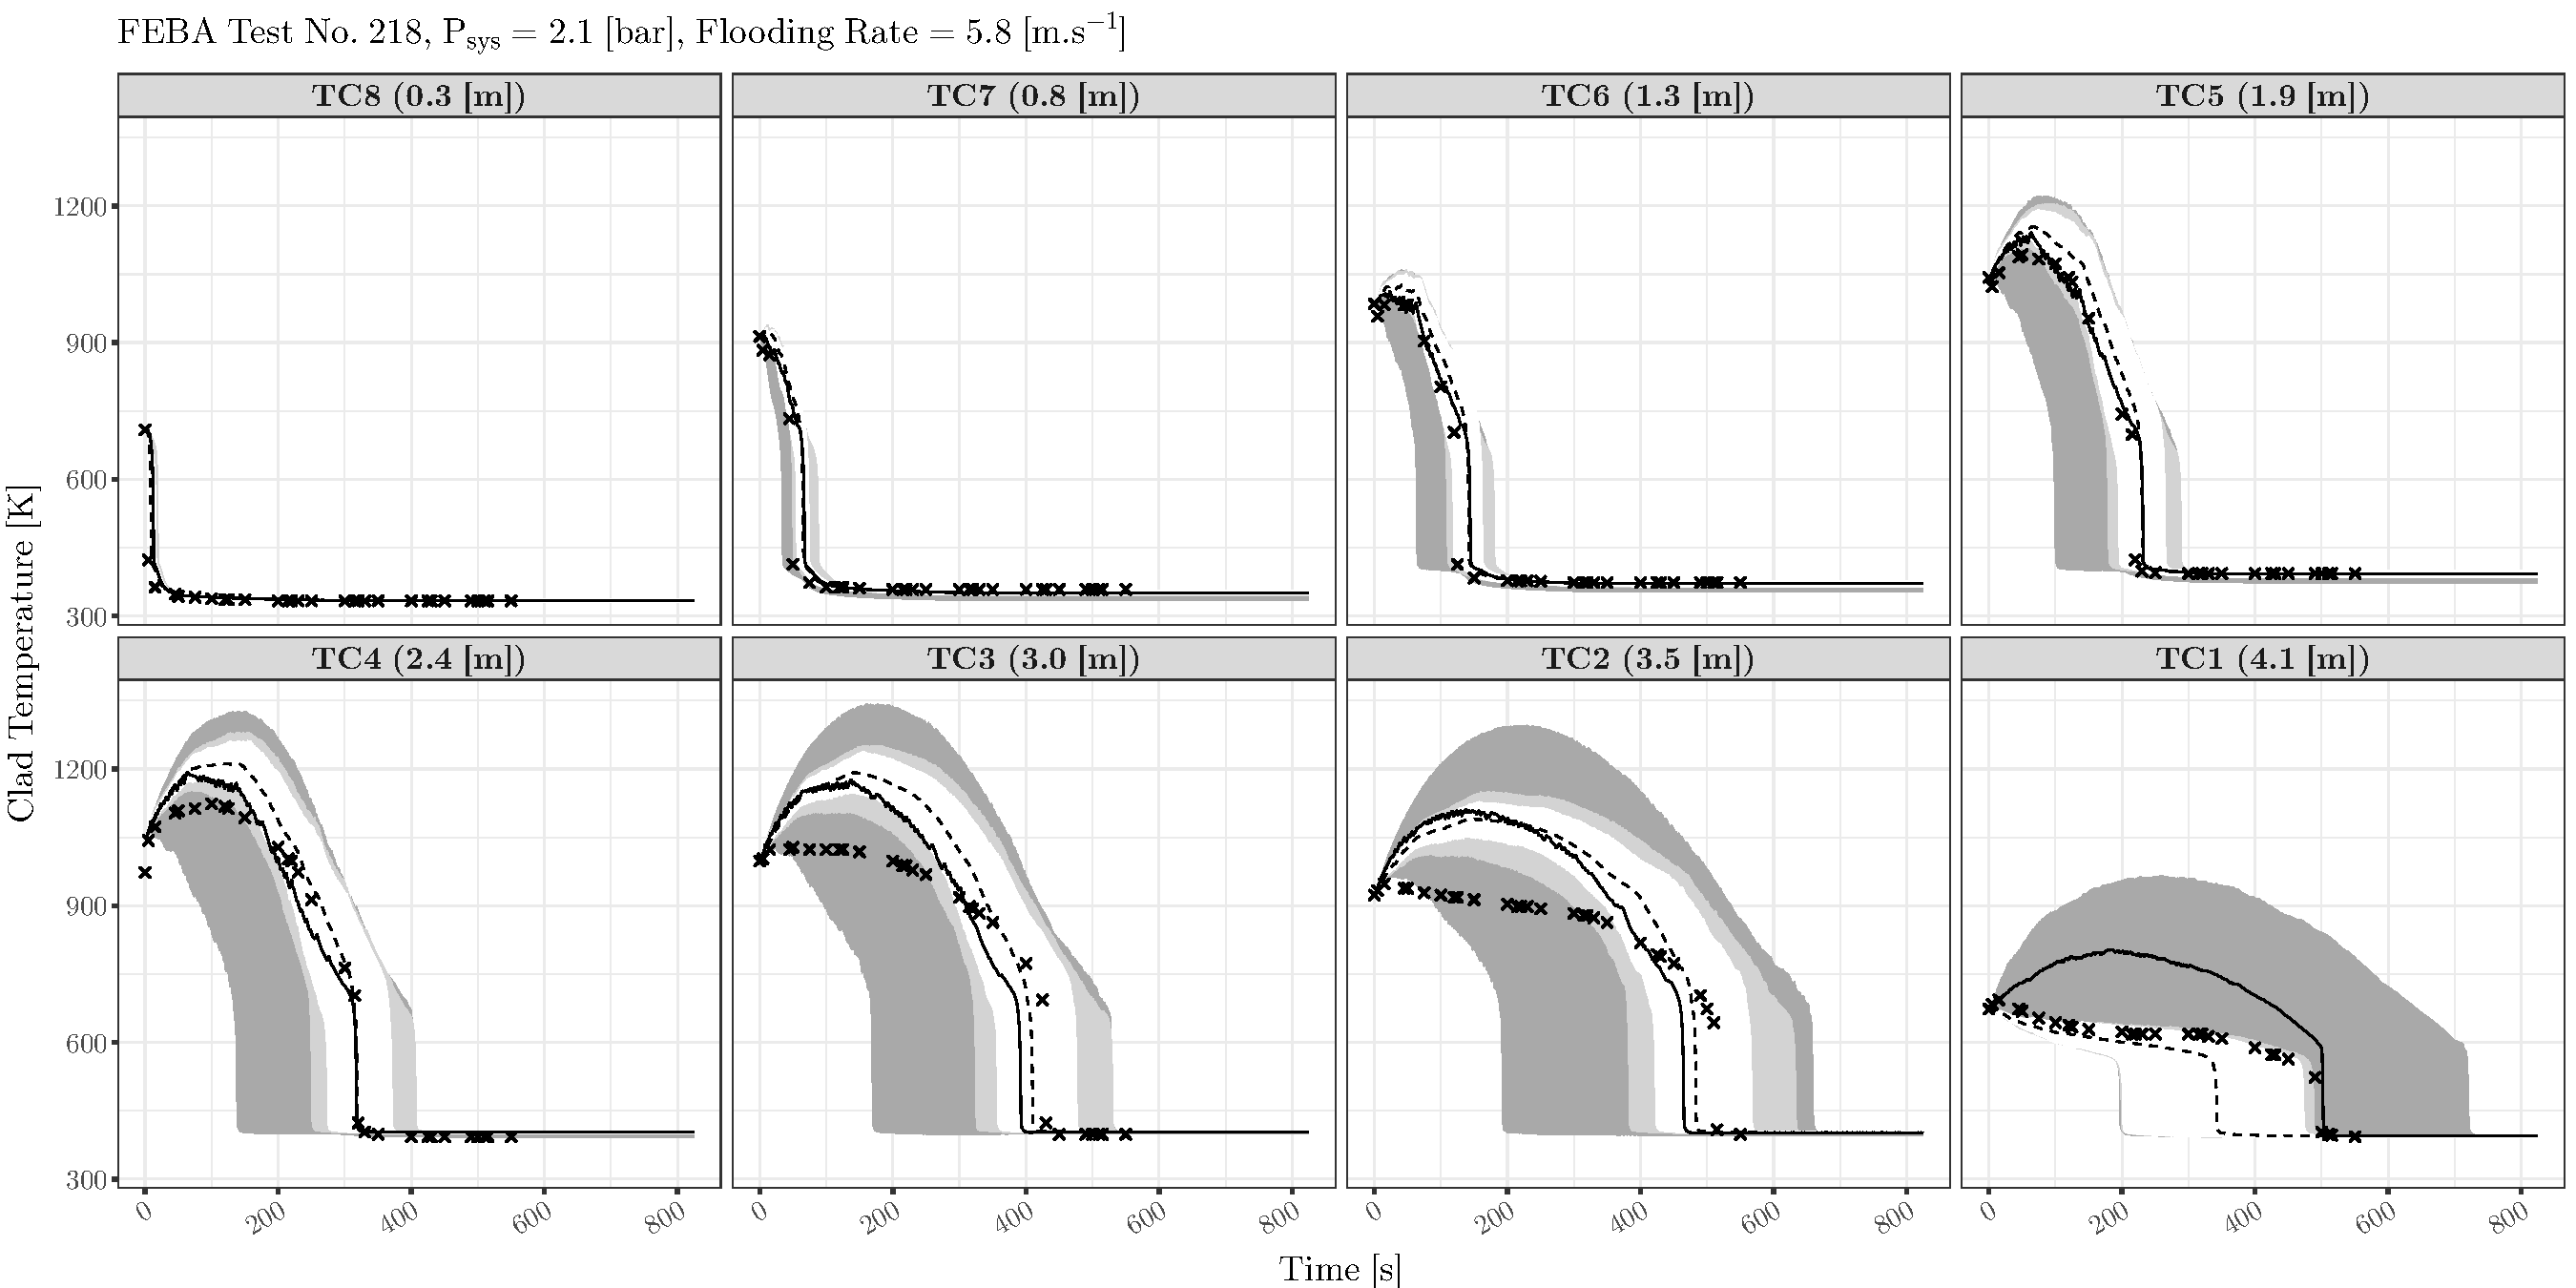
\includegraphics[width=0.90\textwidth]{../figures/chapter5/figures/plotTraceUQPosteriorAllNoDiscNoBCTC218}
		\captionof{figure}[Posterior uncertainty propagation of FEBA Test No. $218$ for the cladding temperature output ($TC$). Calibration without model bias term.]{Uncertainty propagation of the parameters uncertainty of \gls[hyper=false]{feba} Test No. $218$ for the cladding temperature output ($TC$) at different axial locations. The uncertainty bounds refer to the symmetric ($95\%$) probability: dark gray, gray, and light gray correspond to the prior, correlated posterior, and independent posterior samples of the parameters, respectively. Solid lines, dashed lines, and crosses indicate the simulation with the nominal parameters values, the median of the posterior uncertainties, and the experimental data, respectively. Posterior samples from calibration without model bias term.}
	\label{fig:ch5_plot_trace_uq_post_tc_214_nodisc}
\end{sidewaysfigure}
\clearpage
